\chapter{System Architecture and Closed-Loop Design}
\label{ch:arch_design}

\section{System Layered Architecture}
The system is architected as an autonomous, closed-loop Software-Defined Network control platform designed to monitor kernel and physical datapaths, forecast incipient congestion episodes, compute constrained multipath bypasses, install safe OpenFlow 1.3 flow rules, and continuously verify post-reroute telemetry relief.

Figure~\ref{fig:arch_block_diagram} illustrates the end-to-end layered architecture of the platform.

\begin{figure}[H]
  \centering
  \begin{tcolorbox}[colback=codebg,colframe=sdnnavy,arc=3pt,boxrule=1pt,title=\textbf{End-to-End System Layered Architecture}]
  \centering\small\sffamily
  
  \begin{tcolorbox}[colback=white,colframe=sdnblue!50,arc=2pt,boxrule=0.6pt,halign=center,top=3pt,bottom=3pt]
    \textbf{\color{sdnnavy}Layer 5: Visualization \& Human-in-the-Loop Operations}\\[1pt]
    \footnotesize React 18 + TypeScript Console $\cdot$ Canvas Topologies $\cdot$ Strip Charts $\cdot$ LangGraph Agent Modal
  \end{tcolorbox}
  \vspace{-6pt}{\scriptsize\color{sdnblue}$\Updownarrow$ \textit{WebSocket Telemetry Stream (2\,Hz) \& RESTful JWT API}}\vspace{-3pt}
  
  \begin{tcolorbox}[colback=white,colframe=sdnblue!50,arc=2pt,boxrule=0.6pt,halign=center,top=3pt,bottom=3pt]
    \textbf{\color{sdnnavy}Layer 4: Agentic Orchestration \& Decision Plane}\\[1pt]
    \footnotesize LangGraph StateGraph Engine $\cdot$ LLM Cognitive Risk Assessment $\cdot$ OpenRouter API / Deterministic Fallback
  \end{tcolorbox}
  \vspace{-6pt}{\scriptsize\color{sdnblue}$\Updownarrow$ \textit{Internal Python API \& Tool Execution Bus}}\vspace{-3pt}
  
  \begin{tcolorbox}[colback=white,colframe=sdnblue!50,arc=2pt,boxrule=0.6pt,halign=center,top=3pt,bottom=3pt]
    \textbf{\color{sdnnavy}Layer 3: Machine Learning \& Telemetry Analytics}\\[1pt]
    \footnotesize Online Rolling Feature Pipeline $\cdot$ Random Forest Classifier $\cdot$ Calibrated Hazard Probability ($p$)
  \end{tcolorbox}
  \vspace{-6pt}{\scriptsize\color{sdnblue}$\Updownarrow$ \textit{Port Counter Deltas \& Historical Sliding Windows}}\vspace{-3pt}
  
  \begin{tcolorbox}[colback=white,colframe=sdnblue!50,arc=2pt,boxrule=0.6pt,halign=center,top=3pt,bottom=3pt]
    \textbf{\color{sdnnavy}Layer 2: SDN Control Plane (Ryu Framework)}\\[1pt]
    \footnotesize OpenFlow 1.3 Controller $\cdot$ Topology Discovery (LLDP) $\cdot$ Path Computation Engine $\cdot$ MBB Flow Dispatcher
  \end{tcolorbox}
  \vspace{-6pt}{\scriptsize\color{sdnblue}$\Updownarrow$ \textit{OpenFlow 1.3 Southbound Channel (\texttt{OFPT\_PORT\_STATS}, \texttt{OFPFC\_ADD}, \texttt{OFPFC\_MODIFY})}}\vspace{-3pt}
  
  \begin{tcolorbox}[colback=white,colframe=sdnblue!50,arc=2pt,boxrule=0.6pt,halign=center,top=3pt,bottom=3pt]
    \textbf{\color{sdnnavy}Layer 1: Emulated Data Plane (Mininet \cite{lantz2010network} + Open vSwitch + Linux TC)}\\[1pt]
    \footnotesize Open vSwitch Software Switches $\cdot$ Virtual Ethernet Links (\texttt{veth}) $\cdot$ Netem Queue Buffers (100 pkts)
  \end{tcolorbox}
  \end{tcolorbox}
  \caption{Layered architecture of the autonomous closed-loop SDN optimization platform.}
  \label{fig:arch_block_diagram}
\end{figure}

\section{The Five-Stage Control Cycle}
The heartbeat of the platform is the formal closed-loop control cycle, structured into five contiguous operational stages:
\begin{equation}
  \mathcal{C} = \left\langle \text{Observe}, \text{Predict}, \text{Decide}, \text{Reroute}, \text{Verify} \right\rangle
\end{equation}

\subsection{1. Observe (Telemetry Ingestion)}
The controller maintains an asynchronous polling task executing at interval $T_{\text{poll}} = 2.0$\,seconds. For every active switch datapath identifier (DPID) and physical port $p$, the controller constructs an OpenFlow multipart port-statistics request (\texttt{OFPPortStatsRequest}). Upon receiving the \texttt{OFPPortStatsReply}, byte deltas are extracted to compute instantaneous utilization:
\begin{equation}
  R_{\text{tx}}(t) = \frac{(B_{\text{tx}}(t) - B_{\text{tx}}(t - \Delta t)) \times 8}{\Delta t \times 10^6} \quad [\text{Mbps}], \quad U(t) = \frac{R_{\text{tx}}(t)}{C} \times 100 \quad [\%]
\end{equation}

\subsection{2. Predict (Incipient Hazard Inference)}
Instantaneous metrics are pushed into a fixed-size trailing sliding window $\mathcal{W}$ containing $N=12$ samples ($\sim 24$ seconds). Rolling mean, standard deviation, and regression slope ($\text{slope}_U$) are computed. The vector is evaluated by the trained Random Forest classifier $\mathcal{M}_{\text{RF}}$:
\begin{equation}
  p_t = P(\text{Congestion in } [t + 2\text{s}, t + 12\text{s}] \mid \mathbf{x}_t) = \mathcal{M}_{\text{RF}}(\mathbf{x}_t)
\end{equation}
If $p_t \ge 0.50$, the link is flagged as hazardous.

\subsection{3. Decide (Constrained Multi-Path Synthesis)}
The predicted probability $p_t$ is injected as a proactive hazard penalty in the edge cost function:
\begin{equation}
  \text{Cost}(e) = \alpha \cdot \frac{D(e)}{D_{\text{max}}} + \beta \cdot \frac{U(e)}{100} + \gamma \cdot p_t(e)
\end{equation}
where the weighting coefficients are tuned as $\alpha=0.2, \beta=0.3, \gamma=0.5$:
\begin{itemize}[noitemsep]
  \item \textbf{Hazard Weight ($\gamma = 0.5$)}: Prioritizes predictive congestion warnings ($p_t \ge 0.50$), ensuring the path-finding algorithm bypasses links with impending bufferbloat even before physical utilization spikes.
  \item \textbf{Load Weight ($\beta = 0.3$)}: Penalizes instantaneous link utilization $U(e)$, preventing detour flows from shifting onto secondary corridors that already carry substantial traffic.
  \item \textbf{Delay Weight ($\alpha = 0.2$)}: Minimizes propagation delay stretch ($\frac{D(e)}{D_{\text{max}}}$), ensuring the controller prefers low-latency alternate paths while accepting modest hop-count stretch to bypass saturated links.
\end{itemize}
Dijkstra's constrained algorithm computes the optimal alternate detour path $P_{\text{detour}}$.

\subsection{4. Reroute (Make-Before-Break Flow Installation)}
Detour rules are installed using Make-Before-Break semantics (Algorithm~\ref{alg:mbb_box}), pre-programming all downstream switches before shifting ingress traffic.

\subsection{5. Verify (Closed-Loop Affirmation)}
The verify engine monitors subsequent telemetry samples over $T_{\text{verify}} = 4.0$\,seconds. The action is certified \texttt{PASS} if and only if $U_{\text{bottleneck}} < 80\%$ and packet loss $\le 0.05\%$.

\section{Make-Before-Break (MBB) Protocol}
\label{sec:mbb_protocol}
To prevent transient black-holing and micro-loops during path switchover, rules are installed in strict reverse topological order from the destination-adjacent switch back to the ingress switch, accompanied by barrier synchronization requests (\texttt{OFPT\_BARRIER\_REQUEST}).

\begin{tcolorbox}[colback=codebg,colframe=sdnnavy!80,arc=3pt,title=\textbf{Algorithm 1: Make-Before-Break (MBB) Flow-Mod Installation Protocol}]
\label{alg:mbb_box}
\small\sffamily
\textbf{Input}: Detour path $P = \langle s_{\text{in}}, s_1, s_2, \dots, s_k, s_{\text{out}} \rangle$, Match criteria $M$, Priority $p_{\text{high}}$\\
\textbf{Output}: Traffic rerouted onto $P$ with zero transient packet drops or loops\\[0.2cm]
\textbf{Phase 1: Downstream Forward Path Pre-Programming}
\begin{enumerate}[leftmargin=1.5em,noitemsep]
  \item \textbf{for} $i = k$ \textbf{downto} $1$ \textbf{do}:
  \item \quad $\text{dp} \gets \text{GetDatapath}(s_i)$
  \item \quad $\text{out\_port} \gets \text{GetEgressPort}(s_i \to s_{i+1})$
  \item \quad $\text{rule} \gets \text{ConstructFlowMod}(\text{Match}=M, \text{Action}=\text{Output}(\text{out\_port}), \text{Priority}=p_{\text{high}})$
  \item \quad $\text{dp}.\text{send\_msg}(\text{rule})$
  \item \quad $\text{BarrierRequest}(\text{dp})$ \quad \textit{// Enforce hardware TCAM commit before upstream shift}
\end{enumerate}
\textbf{Phase 2: Ingress Switch Flow Redirection}
\begin{enumerate}[leftmargin=1.5em,noitemsep,resume]
  \item $\text{dp}_{\text{in}} \gets \text{GetDatapath}(s_{\text{in}})$
  \item $\text{out\_port}_{\text{new}} \gets \text{GetEgressPort}(s_{\text{in}} \to s_1)$
  \item $\text{ingress\_rule} \gets \text{ConstructFlowMod}(\text{Match}=M, \text{Action}=\text{Output}(\text{out\_port}_{\text{new}}), \text{Priority}=p_{\text{high}})$
  \item $\text{dp}_{\text{in}}.\text{send\_msg}(\text{ingress\_rule})$
  \item $\text{BarrierRequest}(\text{dp}_{\text{in}})$
\end{enumerate}
\textbf{Phase 3: Drain and Safe Rule Teardown}
\begin{enumerate}[leftmargin=1.5em,noitemsep,resume]
  \item $\text{Sleep}(\Delta t_{\text{drain}})$ \quad \textit{// Allow in-flight packets on old path to exit queues}
  \item $\text{RemoveDeprecatedRules}(\text{OldPath}, M)$
\end{enumerate}
\end{tcolorbox}

\section{The Network Topologies Catalog}
The platform incorporates a rich catalog of 10 distinct network architectures (\texttt{future/api/topologies\_catalog.py}), summarized in Table~\ref{tab:topology_summary_ch2}. While all 10 architectures are modeled in the software catalog and supported by the interactive visualization console, empirical 46-run Mininet sweeps were conducted on the canonical Diamond topology to enable controlled, statistically isolated comparisons against baseline routing algorithms.

\begin{table}[H]
  \centering
  \small
  \caption{SDN Network Topology Catalog (10 Architectures).}
  \label{tab:topology_summary_ch2}
  \begin{tabularx}{\textwidth}{l l c c p{2.2cm} X}
    \toprule
    \textbf{ID} & \textbf{Name} & \textbf{Nodes} & \textbf{Links} & \textbf{Bottleneck} & \textbf{Architectural Domain} \\
    \midrule
    \texttt{diamond} & Classic Diamond & 4 Sw / 2 H & 6 & \texttt{s1--s2} (10M) & Canonical 2-path multipath fabric. \\
    \texttt{fat\_tree} & Fat-Tree Clos & 8 Sw / 4 H & 12 & \texttt{a1--c1} (40M) & Hierarchical 2-tier datacenter fabric. \\
    \texttt{spine\_leaf} & Spine-Leaf & 6 Sw / 2 H & 10 & \texttt{lf1--sp1} (25M) & Non-blocking East-West cloud fabric. \\
    \texttt{abilene} & Internet2 Abilene \cite{tipper2009internet2} & 9 Sw / 2 H & 14 & \texttt{DEN--ORD} (10M) & Continental US Wide-Area Network. \\
    \texttt{linear} & Linear Chain & 5 Sw / 2 H & 6 & \texttt{s2--s3} (10M) & Cascading pipeline queue testbed. \\
    \texttt{ring} & Cyclic Ring & 6 Sw / 2 H & 8 & \texttt{r1--r2} (15M) & Fault-tolerant ring with loop guards. \\
    \texttt{grid} & $3 \times 3$ Mesh Grid & 9 Sw / 2 H & 14 & \texttt{g11--g12} (15M) & Multi-hop planar grid network. \\
    \texttt{clos} & 3-Stage Clos & 7 Sw / 2 H & 14 & \texttt{in1--mid1} (20M) & Telecommunications switching fabric. \\
    \texttt{mesh} & Full Core Mesh & 5 Sw / 2 H & 12 & \texttt{m1--m2} (10M) & Fully meshed core transit network. \\
    \texttt{star} & Hub-and-Spoke & 5 Sw / 4 H & 8 & \texttt{hub--sp1} (10M) & Enterprise campus aggregation core. \\
    \bottomrule
  \end{tabularx}
\end{table}

\begin{figure}[H]
  \centering
  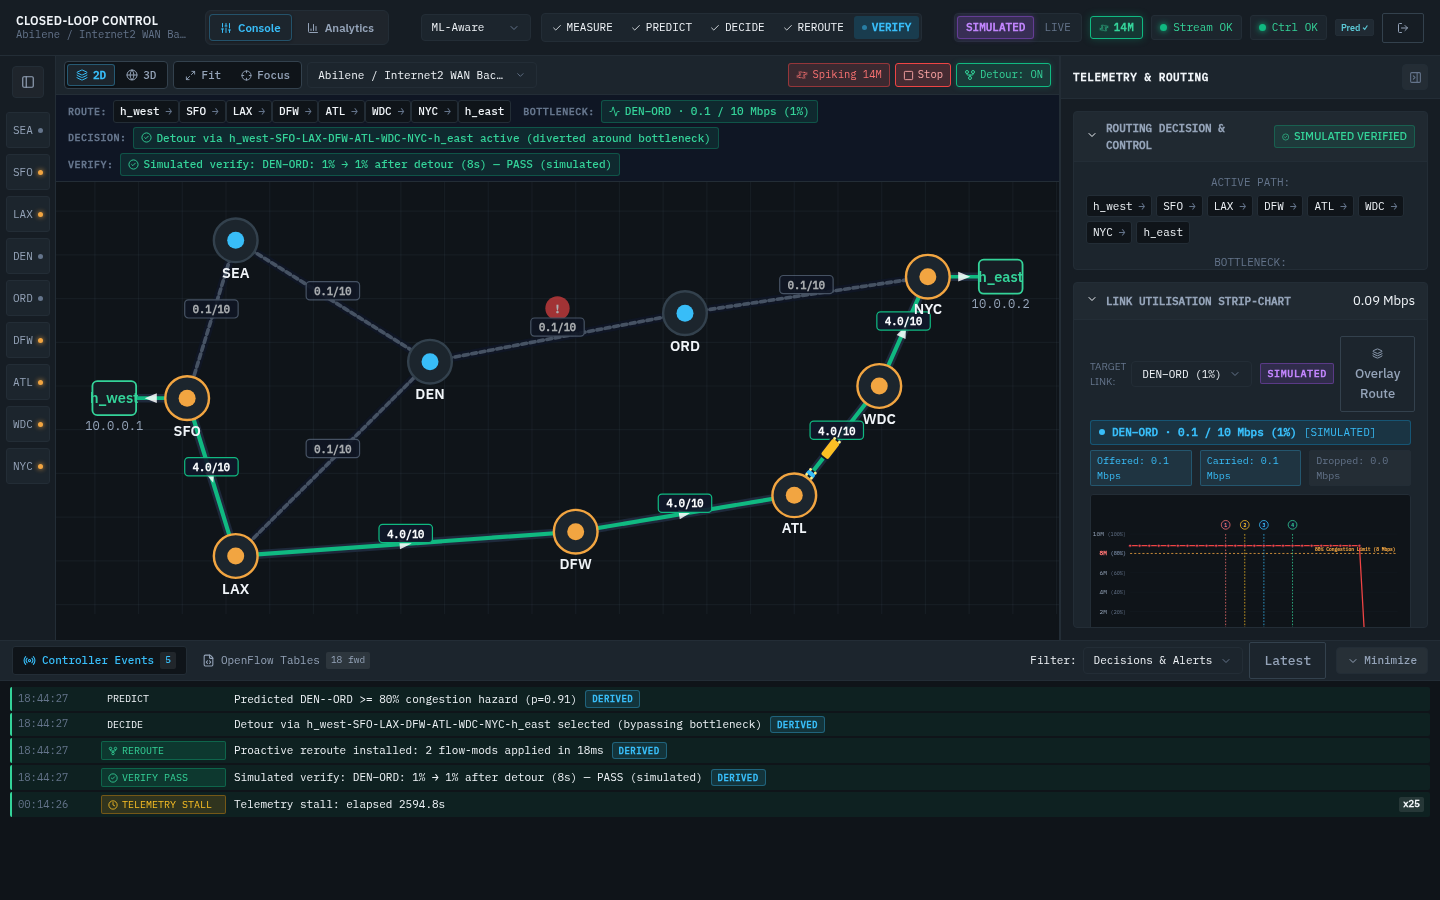
\includegraphics[width=0.82\textwidth]{results/snapshots_ui_fixes/fixed_abilene_detour_pass.png}
  \caption{Internet2 Abilene 9-city continental WAN topology rendered in the interactive visualization console, demonstrating verified Make-Before-Break detour bypass across southern transit links.}
  \label{fig:abilene_console_view_ch2}
\end{figure}
